\section{Justificativa}

Uma pesquisa de 2023 do \gls{sebrae} indica mais de 1,3 milhão de atividades econômicas ligadas a negócios de beleza no Brasil, abrangendo serviços, indústria e comércio, e gerando aproximadamente R\$ 75 bilhões em faturamento anual \cite{sebrae2023forca}. O gráfico abaixo (figura \ref{fig:profissionais_brasil}) demostra o crescimento da quantidade de profissionais no setor da beleza nos últimos anos:

 \begin{figure}[htb]
 	\centering
 	\caption{Profissionais da área da beleza no Brasil 2018–2022}
 	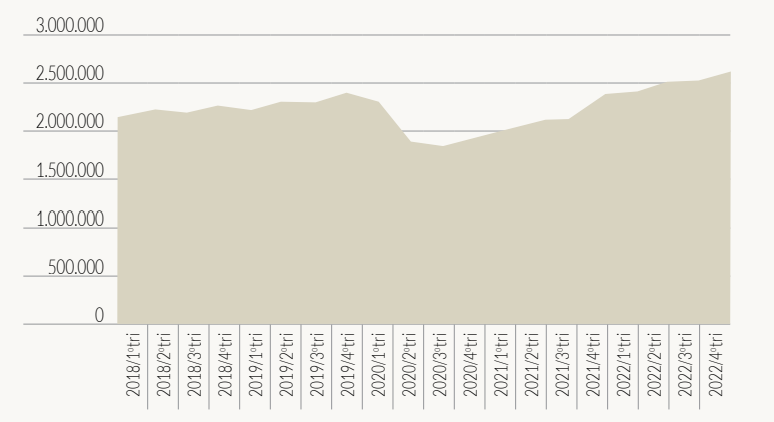
\includegraphics[width=0.9\textwidth]{cap01-Introducao/Images/1.3_grafico_profissionais_brasil}
 	\label{fig:profissionais_brasil}
 	\fonte{\cite{senac_panorama_mercado}}
 \end{figure}
 
 \FloatBarrier
 
Embutido neste crescimento, a maior parte dos profissionais são cabeleireiros, como mostra o gráfico abaixo (\ref{fig:Distribuição_profissionais}):

%inicio de figura
\begin{figure}[htb]
	\centering
	\caption{Distribuição dos profissionais da área da beleza 2018-2021}
	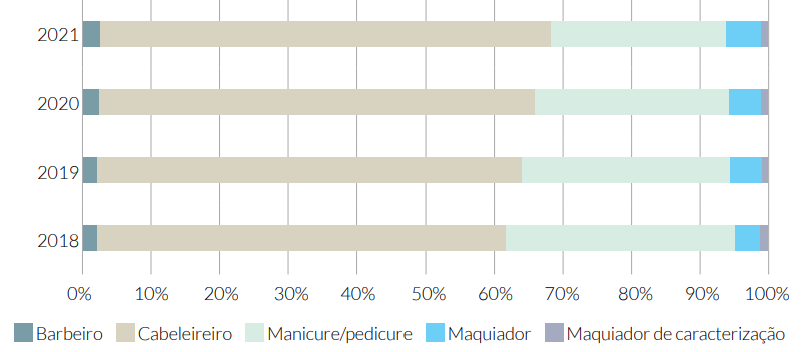
\includegraphics[width=0.9\textwidth]{cap01-Introducao/Images/1.3_grafico_maioria_cabeleireiros}
	\label{fig:Distribuição_profissionais}
	 \fonte{\cite{senac_panorama_mercado}}
\end{figure}

\FloatBarrier

Neste cenário robusto, que movimentou cerca de 27 bilhões de dólares em 2024 \cite{ecommercenapratica2025}, os desafios operacionais crescem cada vez mais: 

\begin{itemize}
	\item Até 30\% do tempo de um pequeno empreendedor é consumido por tarefas administrativas \cite{senac2022};
	\item Taxa média de não comparecimento de clientes atinge 25\% \cite{booksy2022};
	\item Perda de 20\% da receita por não comparecimento \cite{abihpec2021};
	\item Média de 15 horas semanais dedicadas ao controle manual de agenda e finanças \cite{fgv2020};
	\item Insatisfação de 40\% dos clientes devido a falhas de comunicação e alterações de última hora \cite{mindminers2022}.
\end{itemize}

Paralelamente ao crescimento do setor de beleza, o modelo de \emph{coworking}, originado em ambientes de escritório, expandiu-se para salões, permitindo o compartilhamento de espaços e recursos e a redução de custos \cite{sebrae_coworking,sebraesc2025}. Anteriormente à popularização dos \emph{cowrokings} de beleza, os profissionais se distribuiam em diversos locais para economizar recursos, como mostra a figura \ref{fig:Distribuição_locais}:

%inicio de figura
\begin{figure}[htb]
	\centering
	\caption{Distribuição dos profissionais da área da beleza por local de trabalho 2018-2022}
	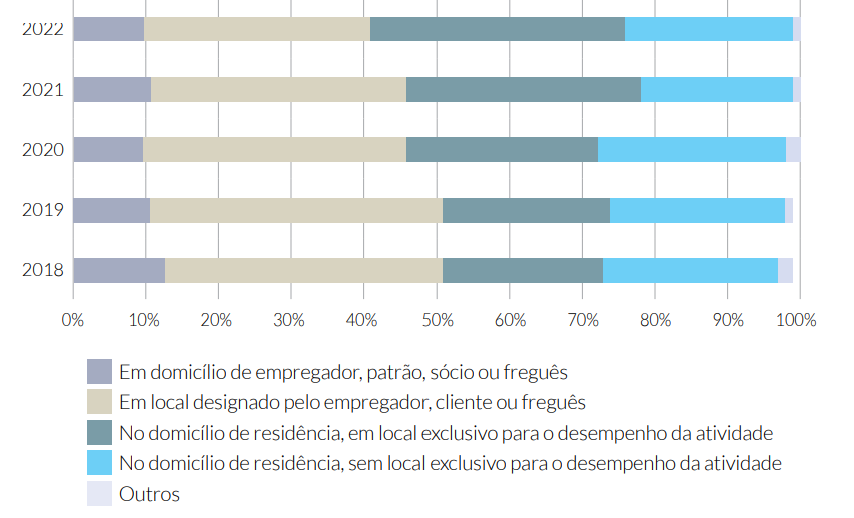
\includegraphics[width=0.9\textwidth]{cap01-Introducao/Images/1.3_local_trabalho_profissionais}
	\label{fig:Distribuição_locais}
	\fonte{\cite{senac_panorama_mercado}}
\end{figure}

\FloatBarrier

Nesse contexto promissor, justifica-se o projeto de extensão \emph{BS Beauty}, destinado a desenvolver uma aplicação \emph{web} customizada para o gerenciamento de salões em modelo \emph{coworking}, sob a coordenação de nossa parceira de extensão Bruna. Ao digitalizar e centralizar processos principais, a BS Beauty empodera pequenos empreendedores reduzindo custos operacionais e minimizando erros humanos, melhora a experiência do cliente, eleva a receita dos profissionais por meio do controle preciso de comissões e frequências, e oferece a oportunidade de \emph{insights} estratégicos através de \emph{dashboards} e relatórios financeiros detalhados. 

Dessa forma, a solução não só supera os problemas de instabilidade e excesso de esforço administrativo, mas também gera valor para todos os envolvidos no salão de beleza. Além disso, como iniciativa de extensão, o projeto permite que os alunos‐desenvolvedores coloquem em prática e melhorem os conhecimentos técnicos e de gestão,  aprendendo com desafios reais de requisitos, usabilidade e performance. Assim, é possível aproximar a graduação das demandas do mercado.


